\section{position}\label{position}

FEATURE IMPORTANCE FOR THE SIGN MODEL

\subsection{Analysis at telescope level}

The random forests for the DISP- and SIGN-prediction get trained on
XXX diffuse gamma events with a 3-fold cross-validation.
The SIGN-model is not needed for this part, but can be useful as 
a cross-check for the LST-mono analysis in section \ref{lst mono part}.

The performance of the models can be gauged by looking at the 
figures \ref{fig:disp_test_perf} for the cross-validated set and 
\ref{fig:disp_test_perf} for the performance our 
pointlike data. Be aware that due to the chosen binning (constant bin width),
the bins do not necessarily contain a comparable amount of events.
This is especially relevant for the highest energy bins.

In both cases we can see that the DISP-model gets rapidly more
powerful with higher energies up until ~\SI{1}{\tera\electronvolt} from 
where on the performance does not improve anymore and in fact seems to decline
again. 

For the diffuse test set, a dip around \SI{3}{\tera\electronvolt}
up to \SI{70}{\tera\electronvolt} can be made out.
This seems to be independent of the binning, as equally filled bins 
do not change this behaviour, see figure \ref{fig:disp_test_perf_2}.

For pointlike gamma events the performance seems to decrease as well, but does not 
recover at the highest energies.
This effect is less prominent with equally filled bins for the pointlike
gammas, see figure \ref{fig:disp_gamma_perf_2}.

The SIGN-model does not saturate like this and improves pretty linear up until
the highest energies. The optimal performance on diffuse events seems 
to be capped earlier than on pointlike events.

\begin{figure}
    \begin{subfigure}{0.45\textwidth}
        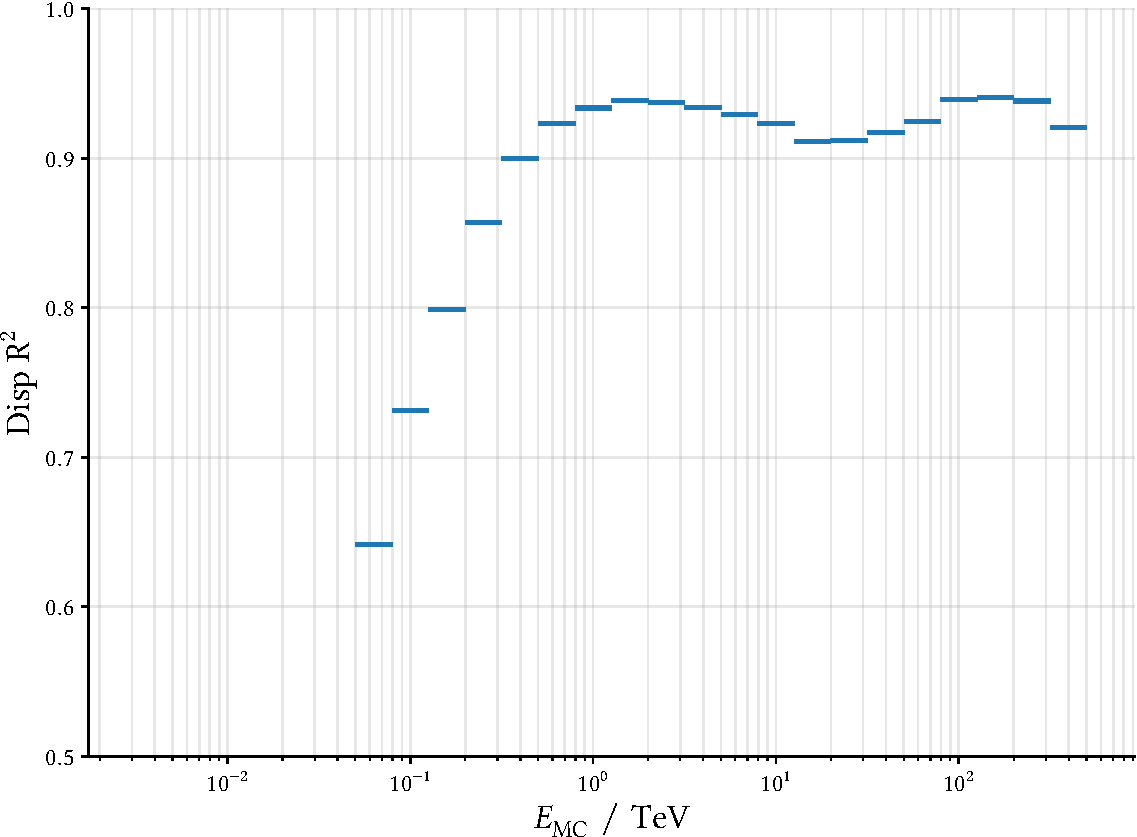
\includegraphics[width=0.9\linewidth]{../analysis/plots/disp_test_r2_equal_sized.pdf} 
        \caption{R2-Score for the DISP-estimation}
    \end{subfigure}
    \begin{subfigure}{0.45\textwidth}
        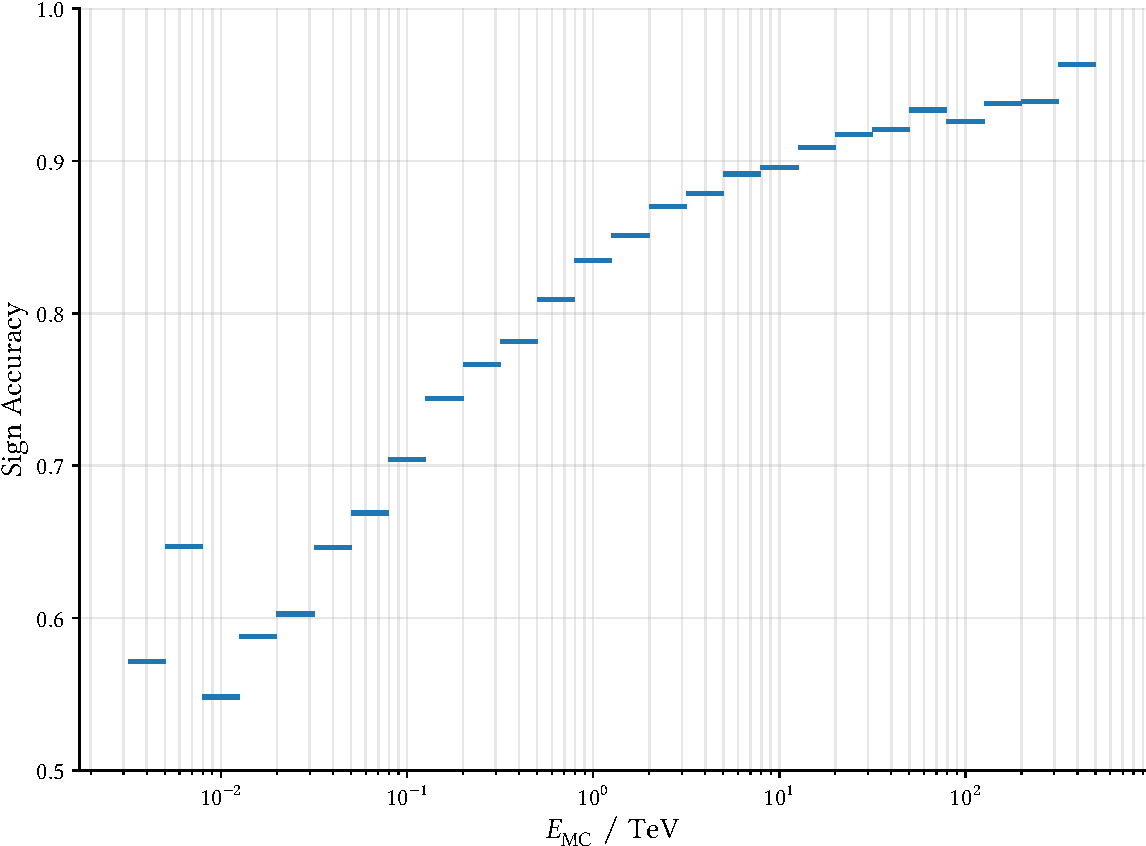
\includegraphics[width=0.9\linewidth]{../analysis/plots/disp_test_acc_equal_sized.pdf}
        \caption{SIGN-accuracy}
    \end{subfigure}
    \caption{Performance of the DISP- and SIGN-estimation algorithm on the test-dataset.}
    \label{fig:disp_test_perf}
\end{figure}

\begin{figure}
    \begin{subfigure}{0.45\textwidth}
        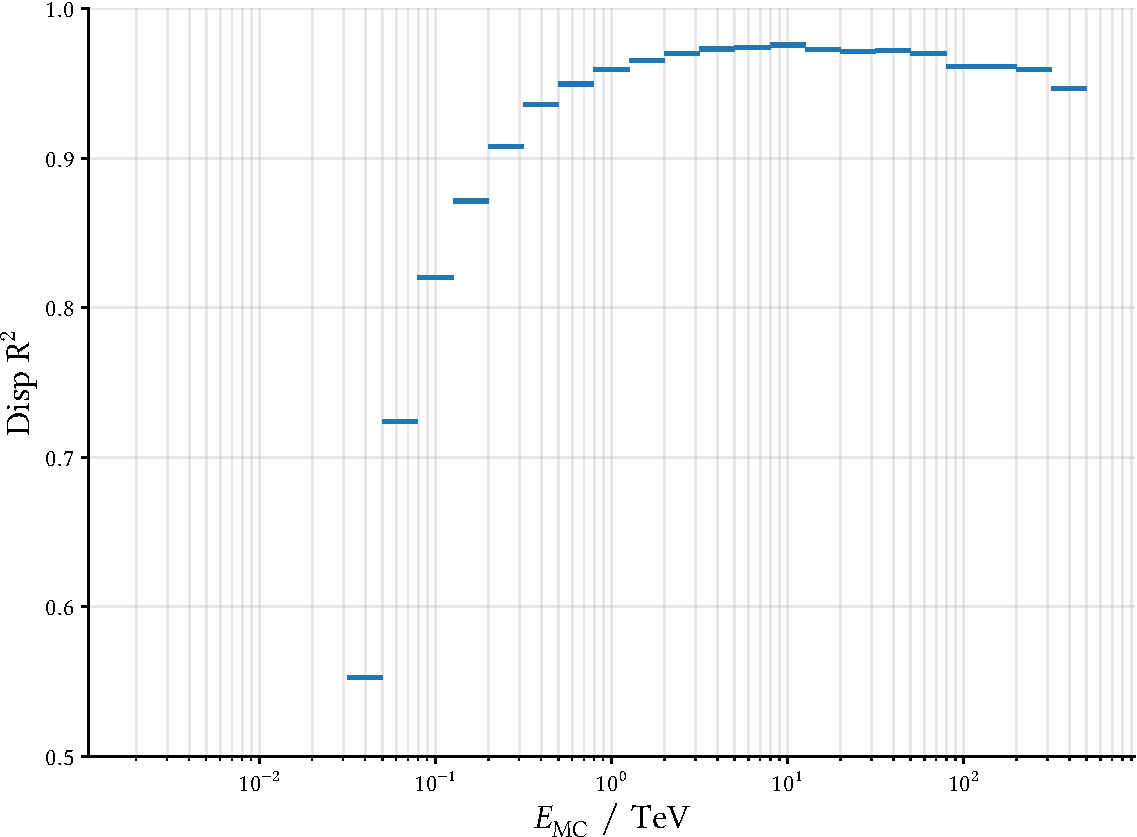
\includegraphics[width=0.9\linewidth]{../analysis/plots/disp_gamma_r2_equal_sized.pdf} 
        \caption{R2-Score for the DISP-estimation}
    \end{subfigure}
    \begin{subfigure}{0.45\textwidth}
        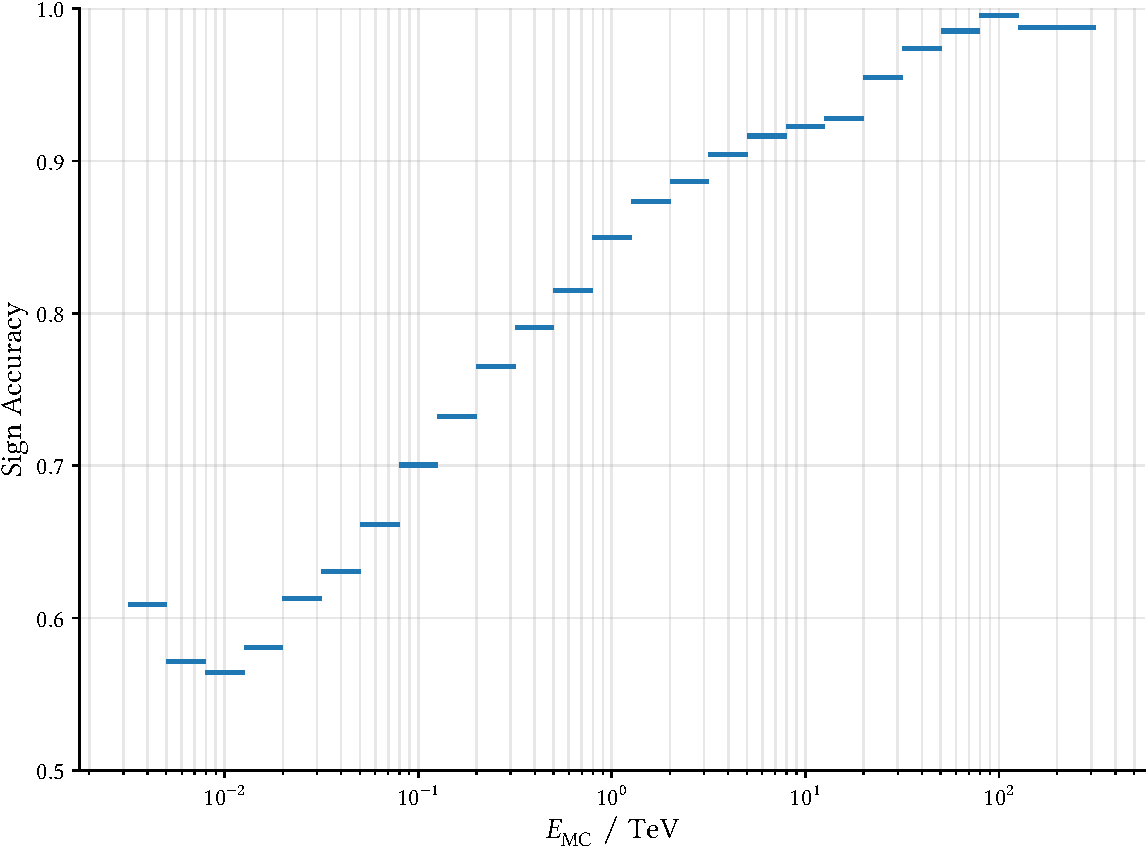
\includegraphics[width=0.9\linewidth]{../analysis/plots/disp_gamma_acc_equal_sized.pdf}
        \caption{SIGN-accuracy}
    \end{subfigure}
    \caption{Performance of the DISP- and SIGN-estimation algorithm on the pointlike dataset..}
    \label{fig:disp_gamma_perf}
\end{figure}

\begin{figure}
    \begin{subfigure}{0.45\textwidth}
        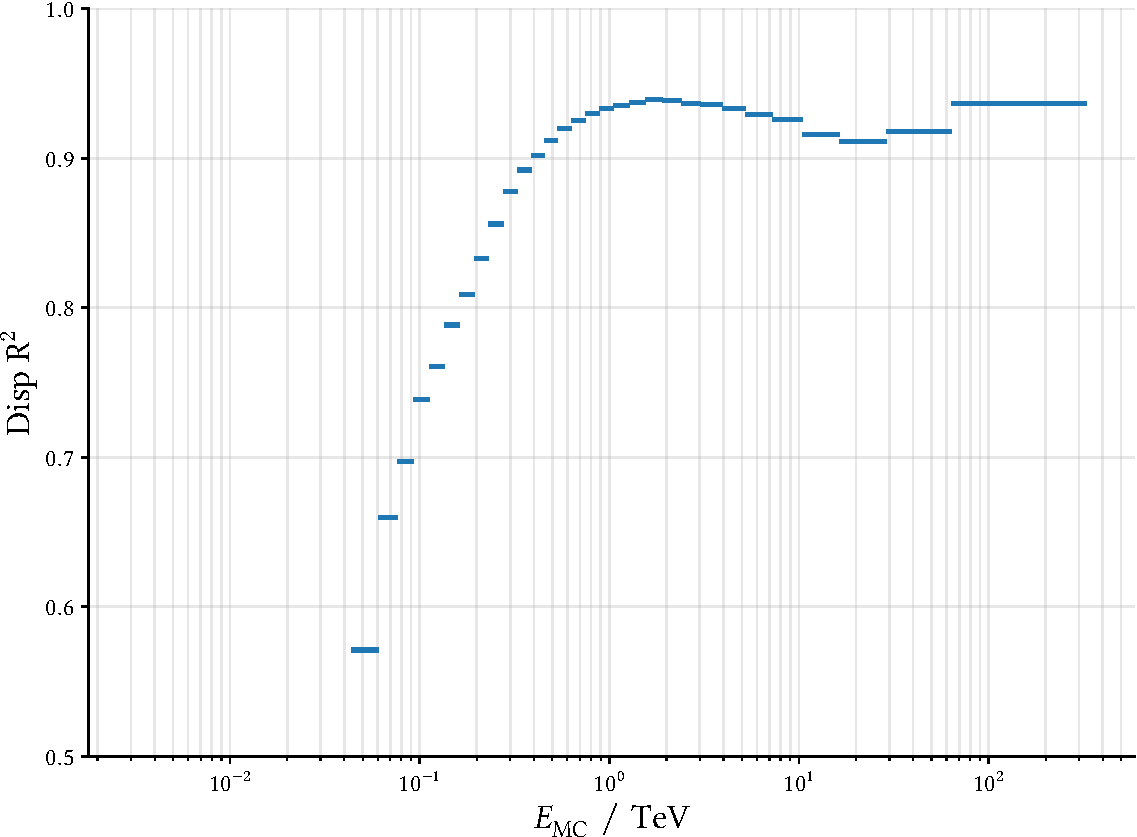
\includegraphics[width=0.9\linewidth]{../analysis/plots/disp_test_r2_equal_filled.pdf} 
        \caption{R2-Score for the DISP-estimation}
    \end{subfigure}
    \begin{subfigure}{0.45\textwidth}
        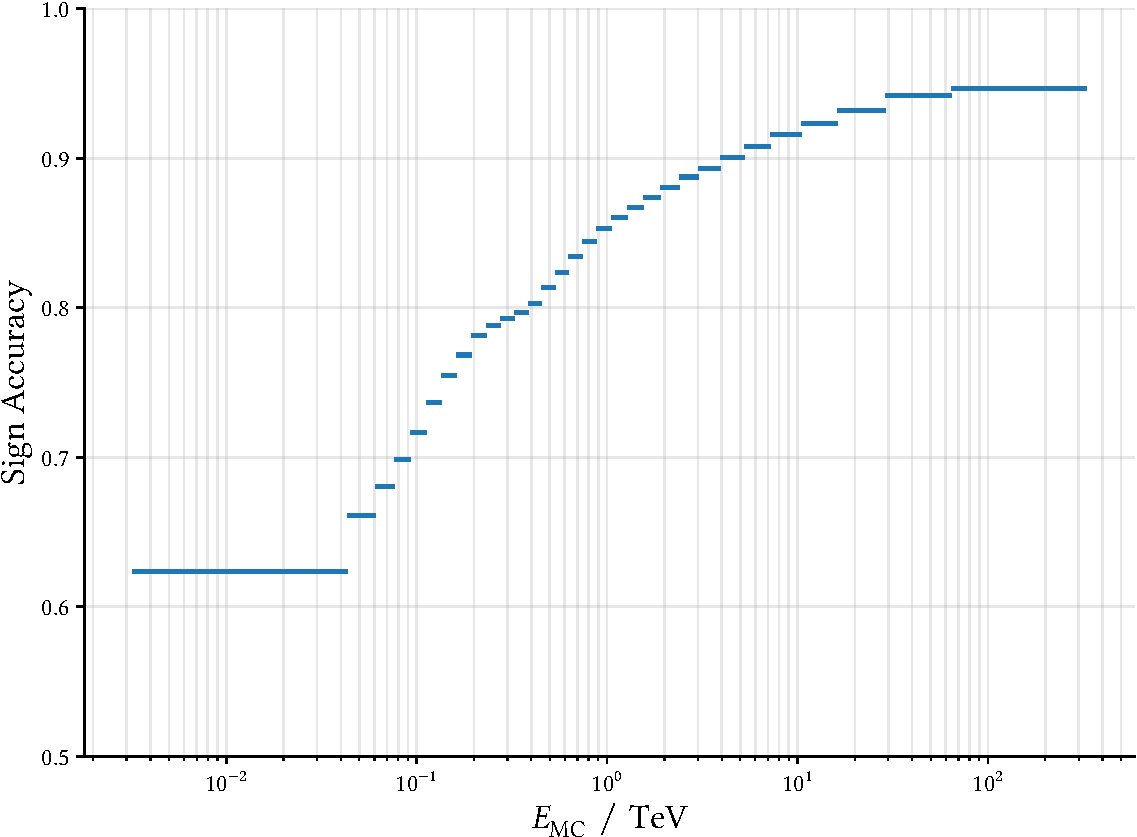
\includegraphics[width=0.9\linewidth]{../analysis/plots/disp_test_acc_equal_filled.pdf}
        \caption{SIGN-accuracy}
    \end{subfigure}
    \caption{Performance of the DISP- and SIGN-estimation algorithm on the test-dataset.}
    \label{fig:disp_test_perf_2}
\end{figure}

\begin{figure}
    \begin{subfigure}{0.45\textwidth}
        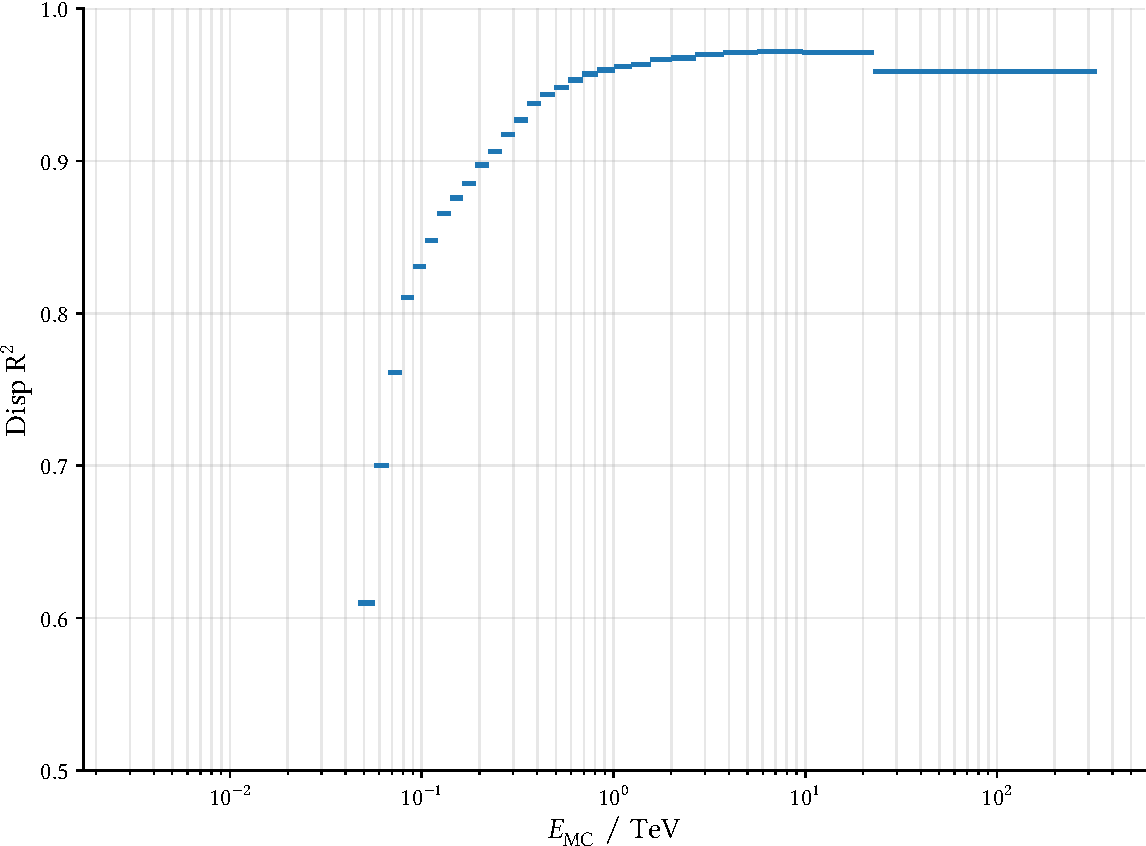
\includegraphics[width=0.9\linewidth]{../analysis/plots/disp_gamma_r2_equal_filled.pdf} 
        \caption{R2-Score for the DISP-estimation}
    \end{subfigure}
    \begin{subfigure}{0.45\textwidth}
        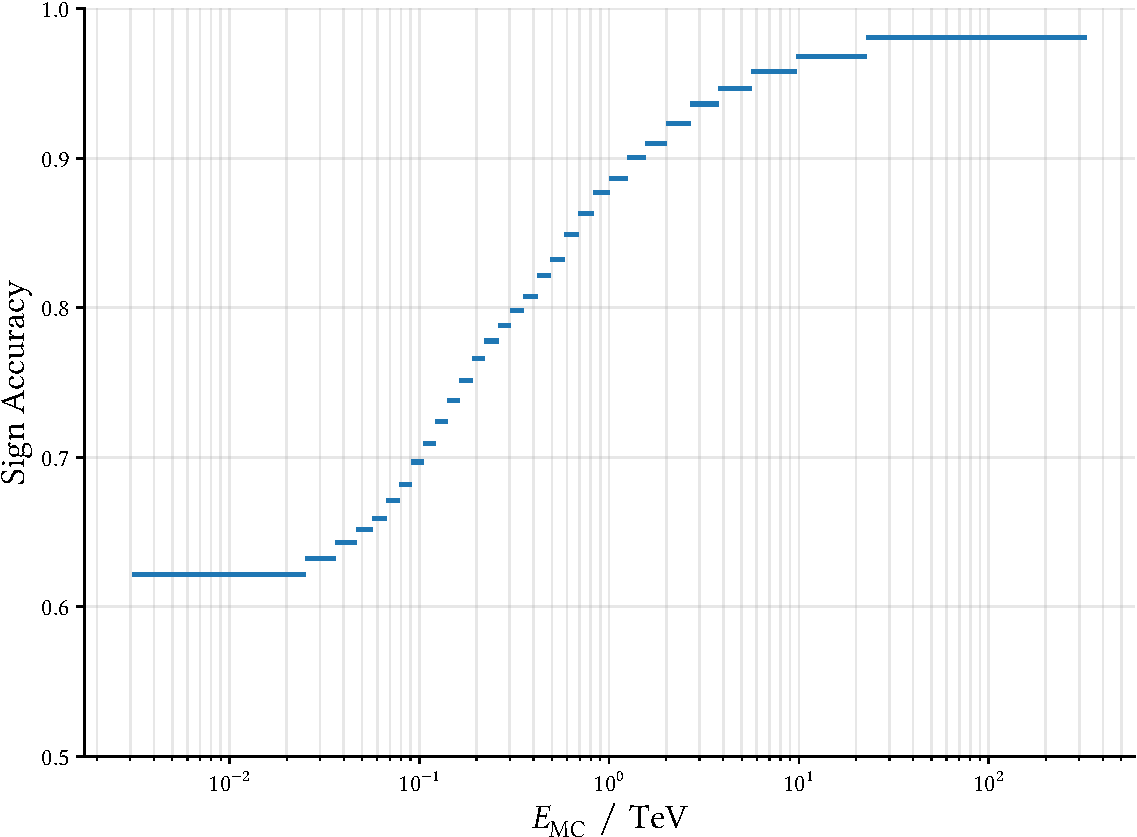
\includegraphics[width=0.9\linewidth]{../analysis/plots/disp_gamma_acc_equal_filled.pdf}
        \caption{SIGN-accuracy}
    \end{subfigure}
    \caption{Performance of the DISP- and SIGN-estimation algorithm on the pointlike dataset..}
    \label{fig:disp_gamma_perf_2}
\end{figure}


Having a look at figure \ref{fig:disp_features} we can learn that 
the stereoscopic features "$distance_to_reconstructed_core_position$"
and $h_max$ have a high influence on the DISP-prediction.
Apart from that the most influence seems to come from the constructed 
feature log\_size\_area, which roughly describes how much light per 
area hit the camera. The timing parameters seem to provide information as 
well. The model also learns on the features focal\_length,  
camera\_type\_id and telescope\_type\_id. This is expected 
behaviour as we have different types of telescopes in the datasets.

\begin{figure}
	\centering
	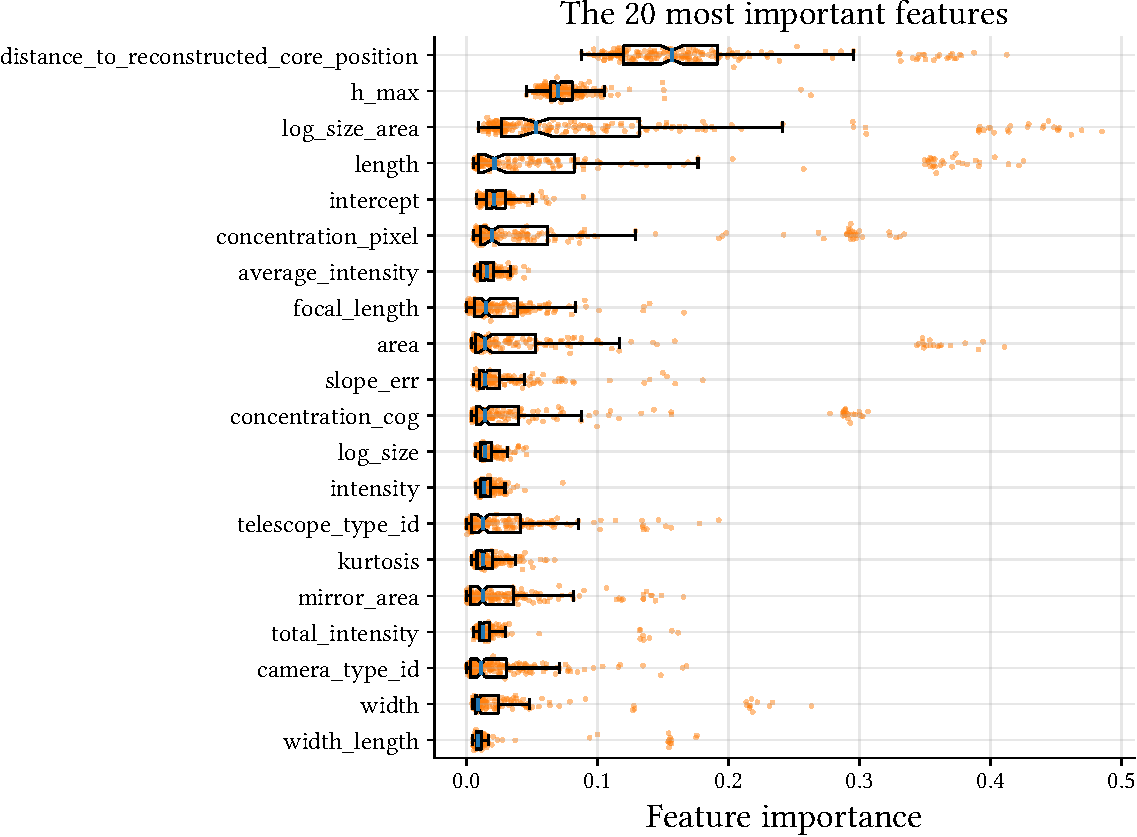
\includegraphics[width=0.8\textwidth]{../analysis/plots/disp_features.pdf}
	\caption{disp features}
	\label{fig:disp_features}
\end{figure}

The final results can be seen in figure \ref{fig:sens_telescope}.
One can derive - in accordance to the previously discussed metrics - 
that the DISP-prediction improves with increasing energies and there are less
missclassified SiGNs at higher energies.
We can also see the saturated DISP-performance at \SI{1}{\tera\electronvolt}.

\begin{figure}
    \centering
    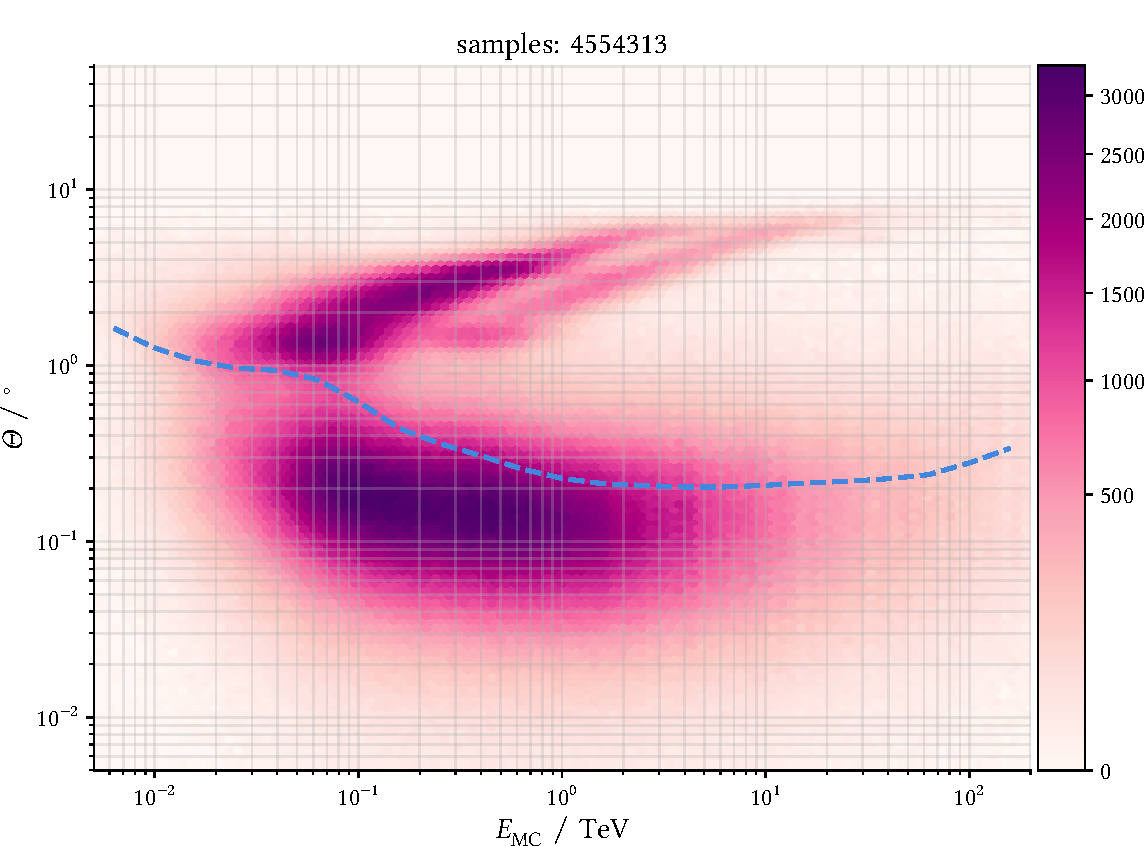
\includegraphics[width=.8\textwidth]{../analysis/plots/gamma/tel_vs_energy.pdf}
    \caption{Per telescope predictions for the source position. The blue-dotted line 
    shows the 68\% containment. A lot of misclassified events at the lower energies
    lead to a second population above the main one below \SI{1}{\degree}.
    The misclassification rate seems to decrease with higher energies 
    in accordance to figures \ref{fig:disp_gamma_perf} and \ref{fig:disp_gamma_perf_2}.
    For very high energies the predictions do not improve despite the lower 
    misclassification rate. This also fits our earlier conclusions.}
    \label{fig:sens_telescope}
\end{figure}


\subsection{Analysis for the stereoscopic array}
MEDIAN NUTZT SIGN -> VORHER KORRIGIEREN UND HIER ERWÄHNEN

As a baseline comparison we compare the median DISP-prediction 
with the results obtained with the Hillas-reconstructor.
Choosing the median should get rid of some misclassification 
problems as events with more correctly than incorrectly 
predicted SIGNs will lead to decent predictions.
These results can be seen in figure \ref{fig:stereo_double_median}
with the 68\% containment of the HillasReconstructor in green 
and the median predictions in blue.
The 2d-histogram in the back refers to the median DISP-predictions,
the HillasReconstructor predictoins are not shown (other than the blue line).

At each energy the Hillas-reconstructor performs considerably better.
One can see that the median predictions do not improve considerably after
\SI{3}{\tera\electronvolt} and gets worse after \SI{20}{\tera\electronvolt}.
The Hillas-reconstructor shows a similar bump at the highest energies.
Due to the low statistics in these regions we can not really tell 
if this shows the limitations of the telescopes sensitivity range 
or if there are just some hard-to-reconstruct events in there. 

The HillasReconstructor also shows a short bump in the range of \SI{200}{\giga\electronvolt}
to \SI{1}{\tera\electronvolt}. 
This has been observed earlier and seems to correlate with 
a lot of low multiplicity events in the crossover region from LSTs to MSTs \cite{????}.

Looking at the multiplicity we can conclude that the median predictions
do not scale as well with higher multiplicities.

\begin{figure}
    \centering
    \begin{subfigure}{0.75\textwidth}
        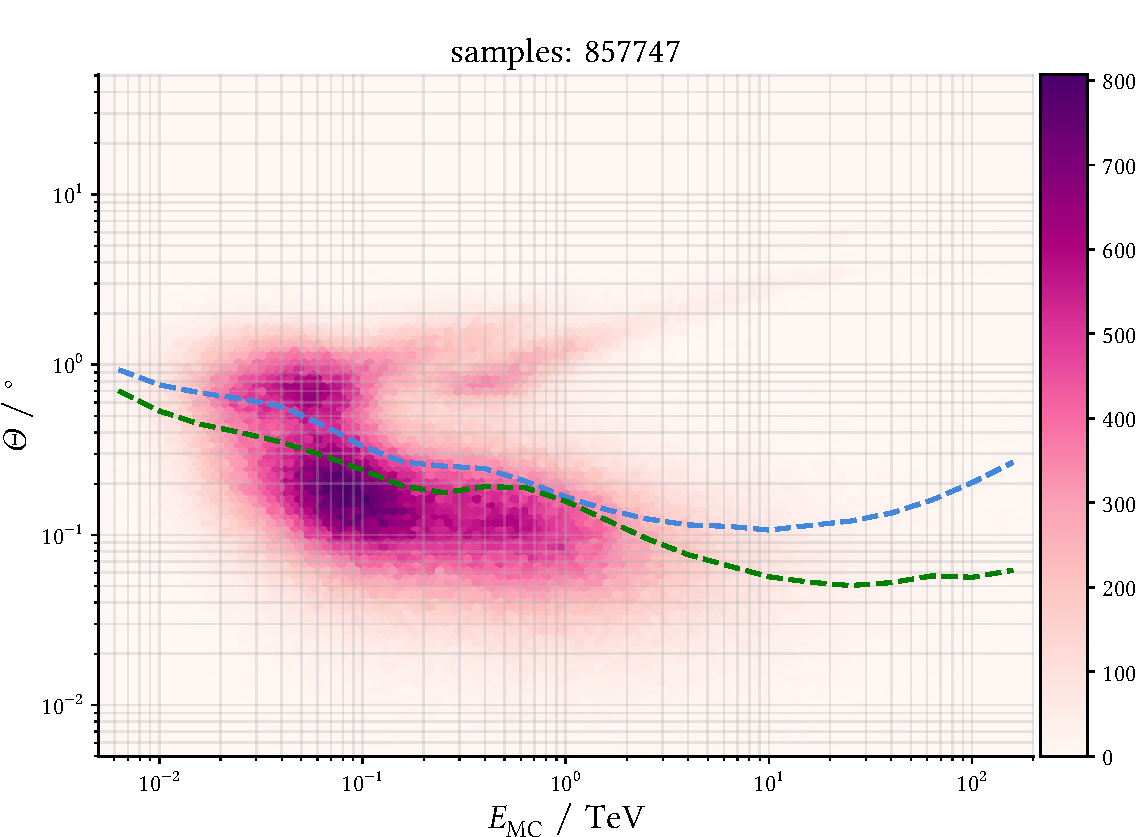
\includegraphics[width=\linewidth]{../analysis/plots/gamma/median_vs_energy.pdf} 
        \caption{Distance to true position against energy}
    \end{subfigure}
    \begin{subfigure}{0.75\textwidth}
        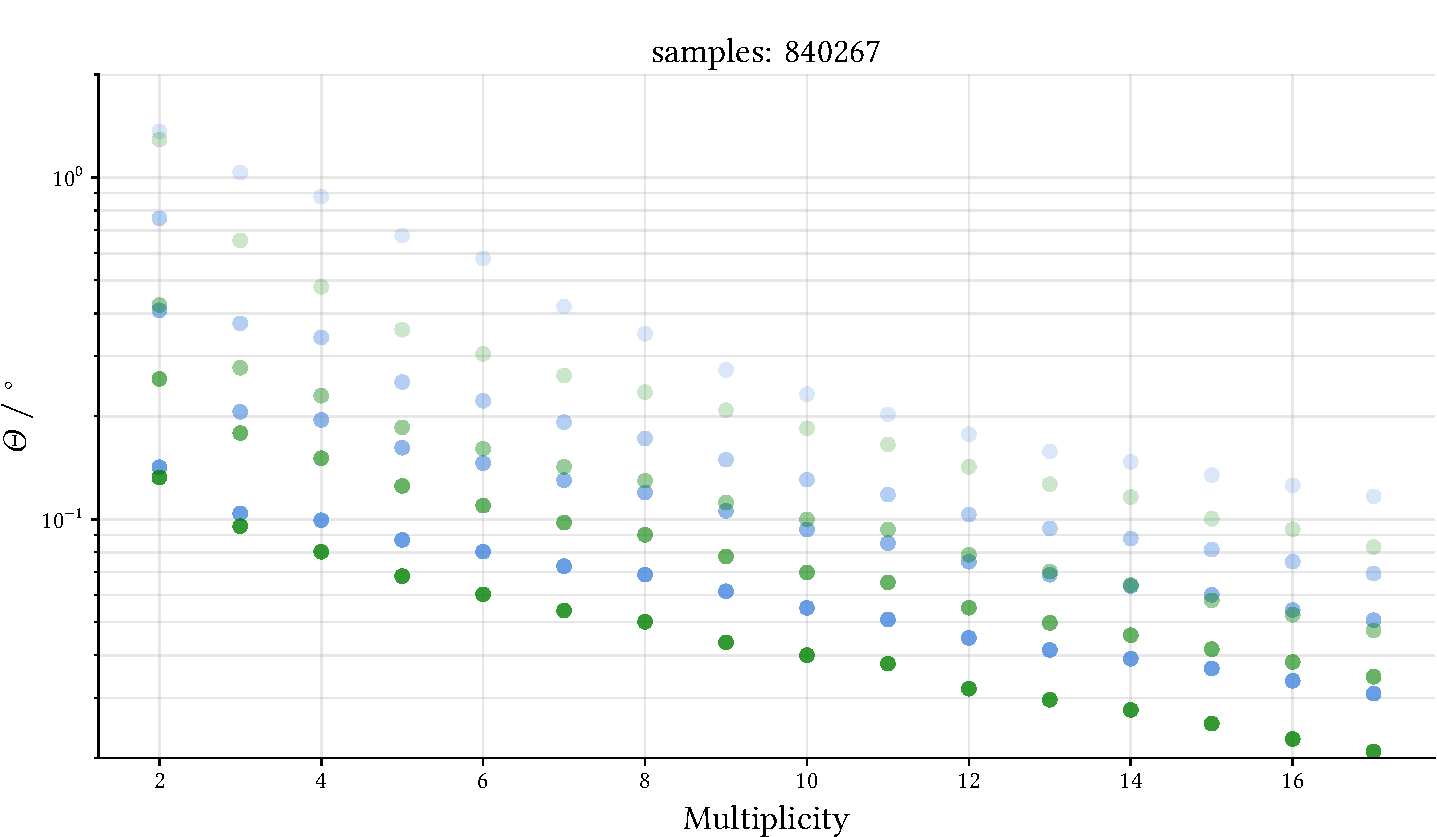
\includegraphics[width=\linewidth]{../analysis/plots/gamma/median_vs_multi_comp.pdf}
        \caption{Distance to true position against event multiplicity}
    \end{subfigure}
    \caption{Performance of the median telescope prediction compared 
    against the results of the HillasReconstructor. 
    Left: Binned results from the median DISP-predictions. The blue line shows the 
    68\% containment of these results. The green line refers to the 
    results of the HillasReconstructor which are not shown otherwise.
    Right: Performance against event multiplicity. Both algorithms requires 
    multiplicities $\geq 2$. Higher multiplicity events are cut off, because 
    statistic is low and the emphasis lies on the lower multiplicity events.
    Blue and green refer to the median predictions and the HillasReconstructor predictions.
    The different lines refer to the 25,50,68 and 90\% percentiles with 
    lowering alpha.
    The median predictions are worse at every multiplicity.}
    \label{fig:stereo_double_median}
\end{figure}

The results of the more sophisticated DISP-approach can be seen in figure \ref{fig:stereo_double_magic}.
Compared to figure \ref{fig:stereo_double_median} the completely misreconstructed events are almost
gone and the 68\% percentile is much improved throughout the complete energy range besides 
the very highest energies. At this point the DISP-error is probably limiting and the 
Hillas-reconstructor leads to much better results.
At the lower energy range our approach seems to be working pretty well, 
slightly outperforming the Hillas-reconstructor, especially 
where the HillasReconstructor shows bumps.

When looking at the multiplicity-plot, we see a similar picture as before but with 
better results. At high event multiplicities $\ge 36$ the Hillas-reconstructor 
leads to better results. Improvements can be seen especially at 2- and 3-multiplicity 
events. In the case of 2 telescopes the iterative approach is identical to the 
Magic-method we based the implementation on.
The Hillas-reconstructor on the other hand does not work too well with 2 
triggered telescopes, with 3 triggered telescopes leading to much better results 
already especially at the 90\% percentile.


\begin{figure}
    \centering
    \begin{subfigure}{0.75\textwidth}
        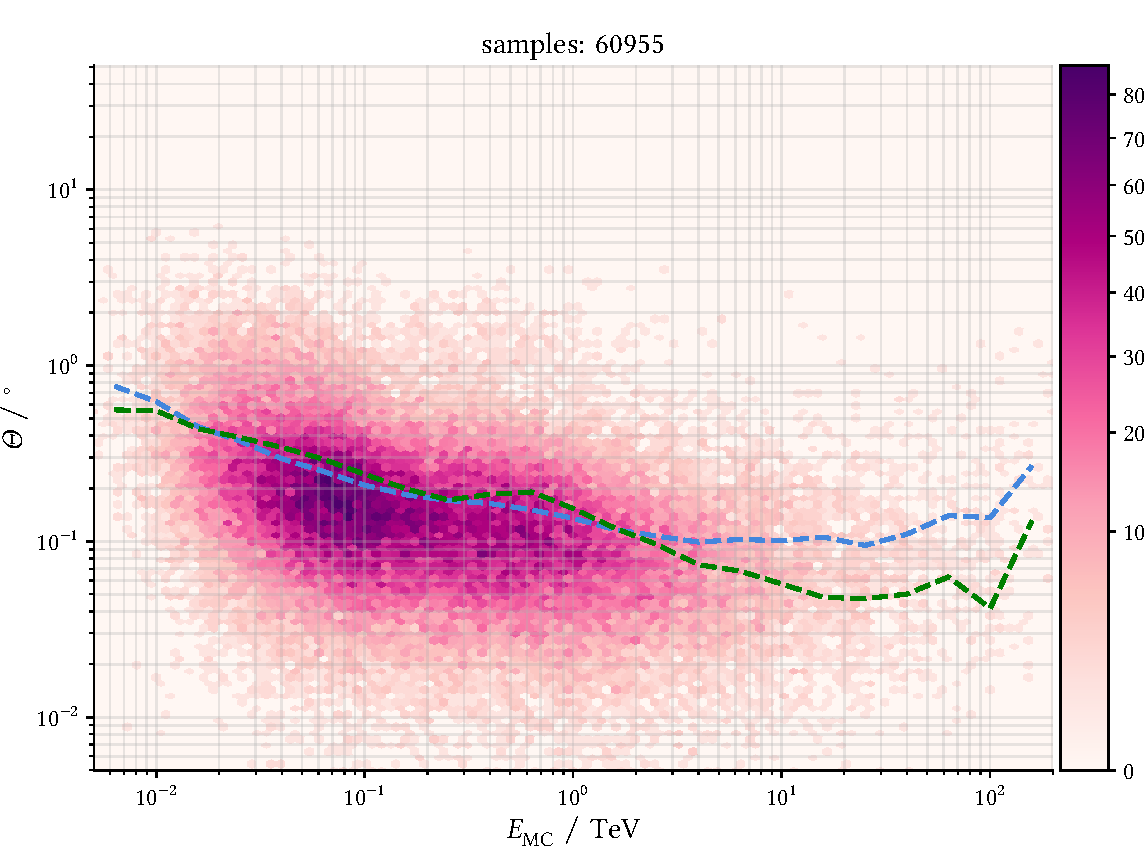
\includegraphics[width=\linewidth]{../analysis/plots/gamma/pairwise_median_100_vs_energy.pdf} 
        \caption{Distance in degree against energy}
    \end{subfigure}
    \begin{subfigure}{0.75\textwidth}
        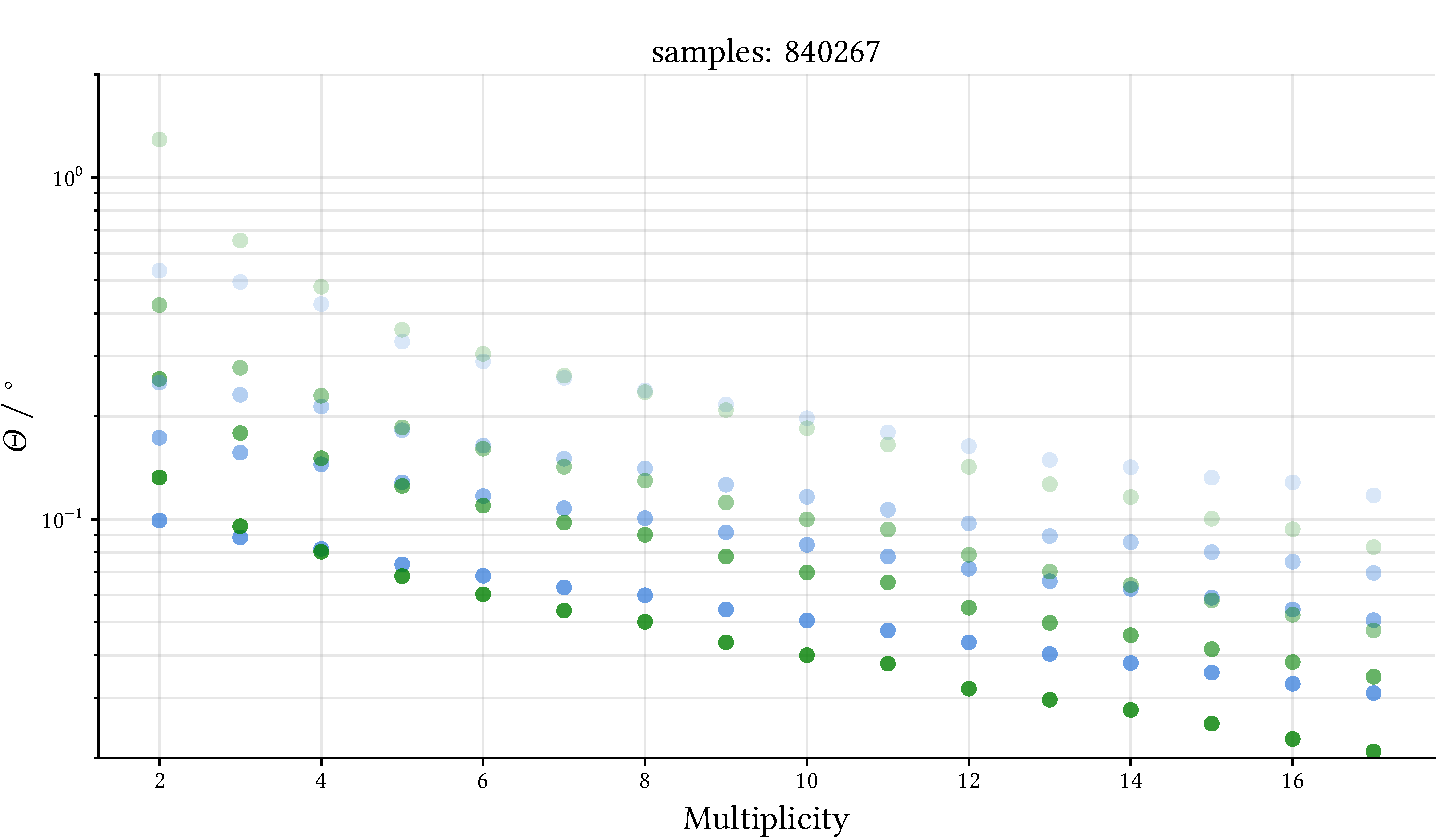
\includegraphics[width=\linewidth]{../analysis/plots/gamma/pairwise_median_100_vs_multi_comp.pdf}
        \caption{Distance in degree against multiplicity}
    \end{subfigure}
    \caption{Performance of the combined DISP-predictions as per our iterative approach
    compared against the results of the HillasReconstructor.
    Left: Binned results from the iteratively combined DISP-predictions.
    The blue line shows the 
    68\% containment of these results. The green line refers to the 
    same results of the HillasReconstructor as in figure \ref{fig:stereo_double_median} 
    which are not included in the binned results.
    Right: Performance against event multiplicity. Both algorithms requires 
    multiplicities $\geq 2$. Higher multiplicity events are cut off, because 
    statistic is low and the emphasis lies on the lower multiplicity events.
    Blue and green refer to the median predictions and the HillasReconstructor predictions.
    The different lines refer to the 25,50,68 and 90\% percentiles with 
    lowering alpha.
    For low multiplicities the combined DISP-predictions are superiour, 
    for high multiplicities the HillasReconstructor results win out.
    The breakeven point seems to be at 4-6 telescopes, depending on 
    which percentiles have more weight to the analysis.}
    \label{fig:stereo_double_magic}
\end{figure}


\section{Hadroness Cut}

In a analysis of real data, some legitimate events usually get discarded
in the gamma-/hadron-separation step.
Assuming that the misclassified events are in some way non regular, it might be 
justified to assume that these events also behave abnormal during the reconstruction of 
the source position. Discarding these events could thus improve the overall 
predictions.

Based on the performance of the gamma-/hadron-separation model (see figure \ref{add that earlier})
we set the gammaness cut at XXX.
This is done purely based on heuristics and does not involve any detailed analysis.

With this cut XXX events or XXX\% of the events remain.

We apply the same model as earlier and compare the results to the HillasReconstructor
again. IRGENDWIE QUANTIFIZIEREN -> THETA**2 VERTEILUNGEN FÜR ALLE ENERGIEN PLOTTEN UND 68\% ANSCHAUEN?


\begin{figure}
    \centering
    \begin{subfigure}{0.75\textwidth}
        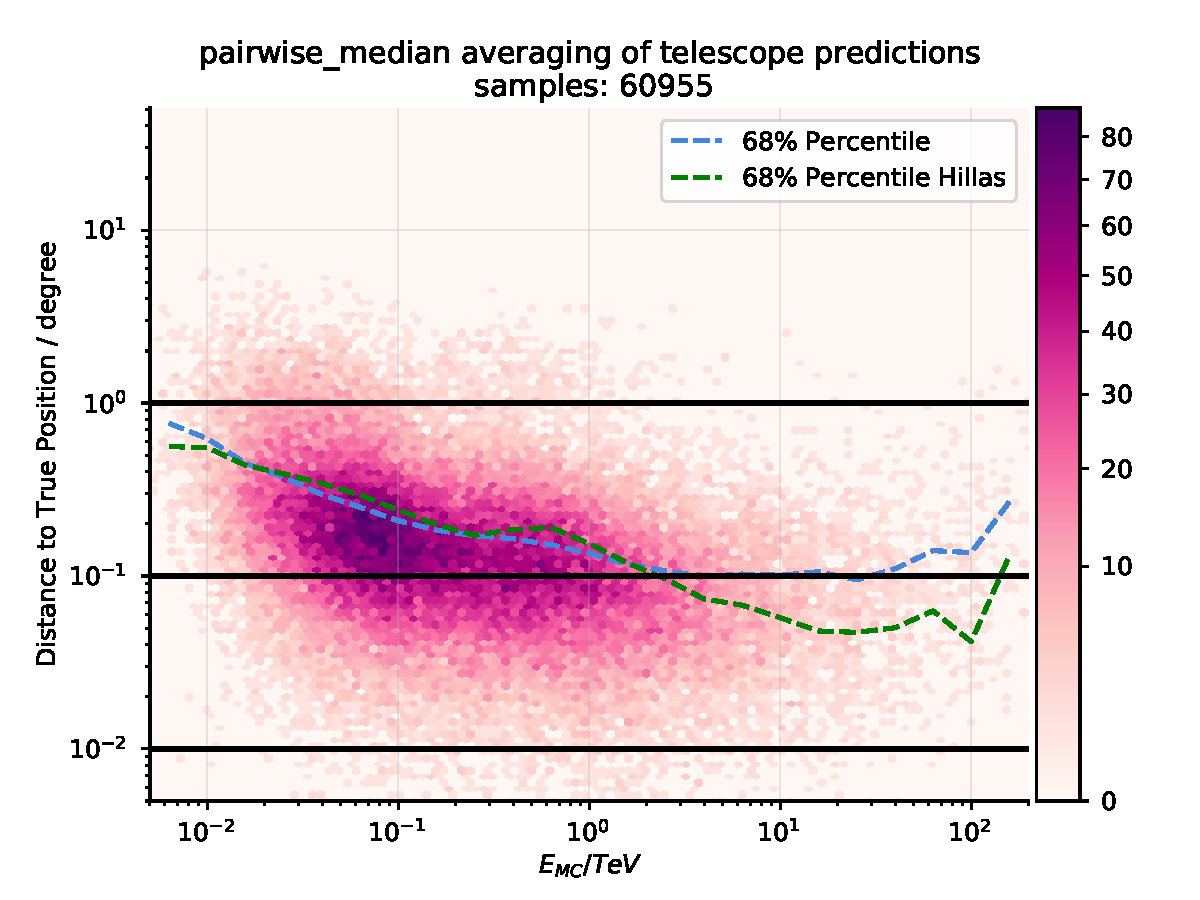
\includegraphics[width=\linewidth]{../analysis/plots/gamma_cut/pairwise_median_100_vs_energy.pdf} 
        \caption{Distance in degree against energy}
    \end{subfigure}
    \begin{subfigure}{0.75\textwidth}
        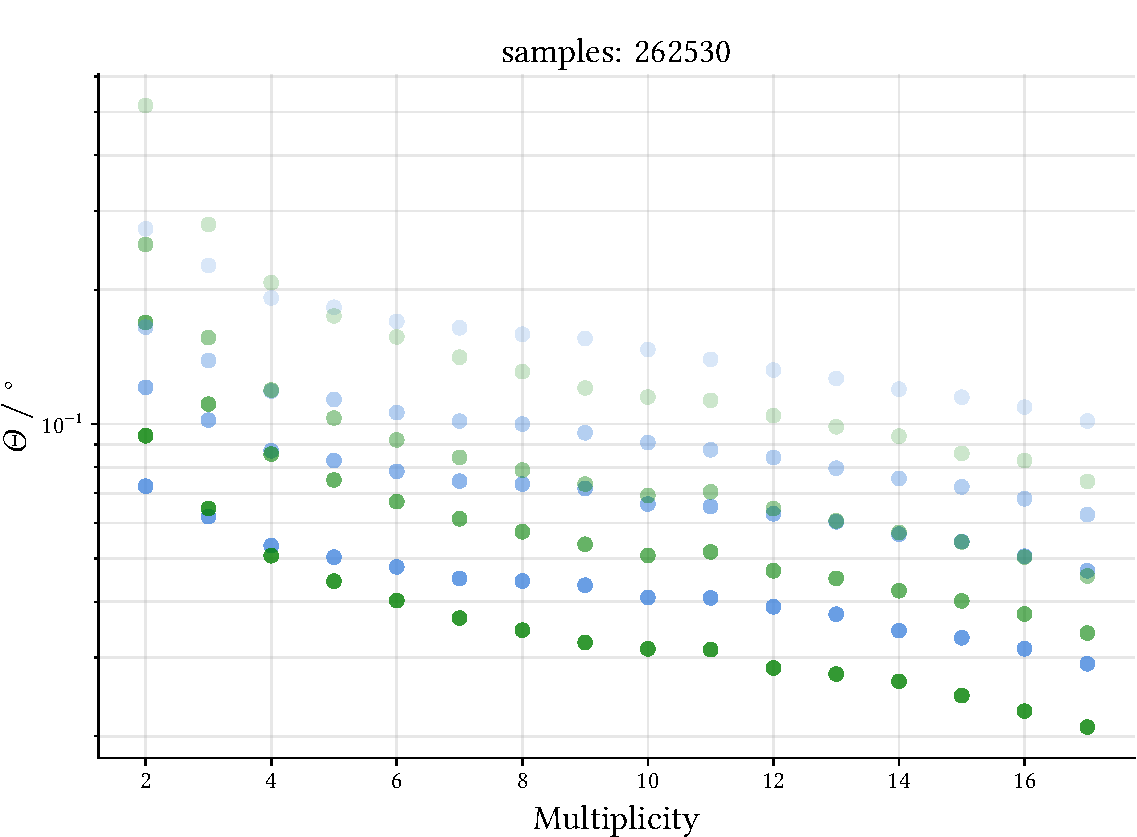
\includegraphics[width=\linewidth]{../analysis/plots/gamma_cut/pairwise_median_100_vs_multi_comp.pdf}
        \caption{Distance in degree against multiplicity}
    \end{subfigure}
    \caption{Performance of the superduper compared 
    against the Hillas-Reconstructor. Median in Blue, Hillas in green
    Actually better, but in the extreme regions where statistics is low as well.}
    \label{fig:stereo_double}
\end{figure}


-> bringt nichts?


\section{LST only}
To simulate early operation stages where the LST1 is the only fully functional 
telescope, the analysis is limited to only the single LST with 
the telescope\_id 4.

This means that we do not have a baseline Hillas Reconstructor as we can not use
stereoscopy and each array event holds exactly one telescope event.
We expect to
get a similar sensitivity as in the earlier figure \ref{fig:sens_telescope}.

We also try to limit the training data on this particular telescope.
This will leave us with far less training samples, but hopefully
a better model?????

HOW DOES THE PERFORMANCE CHANGE?
THIS REQUIRES MORE EVENTS AND MAYBE MORE LSTS FOR TRAINING?
COMPARE TO APPLYING THE NORMAL MODEL

\begin{figure}
    \begin{subfigure}{0.45\textwidth}
        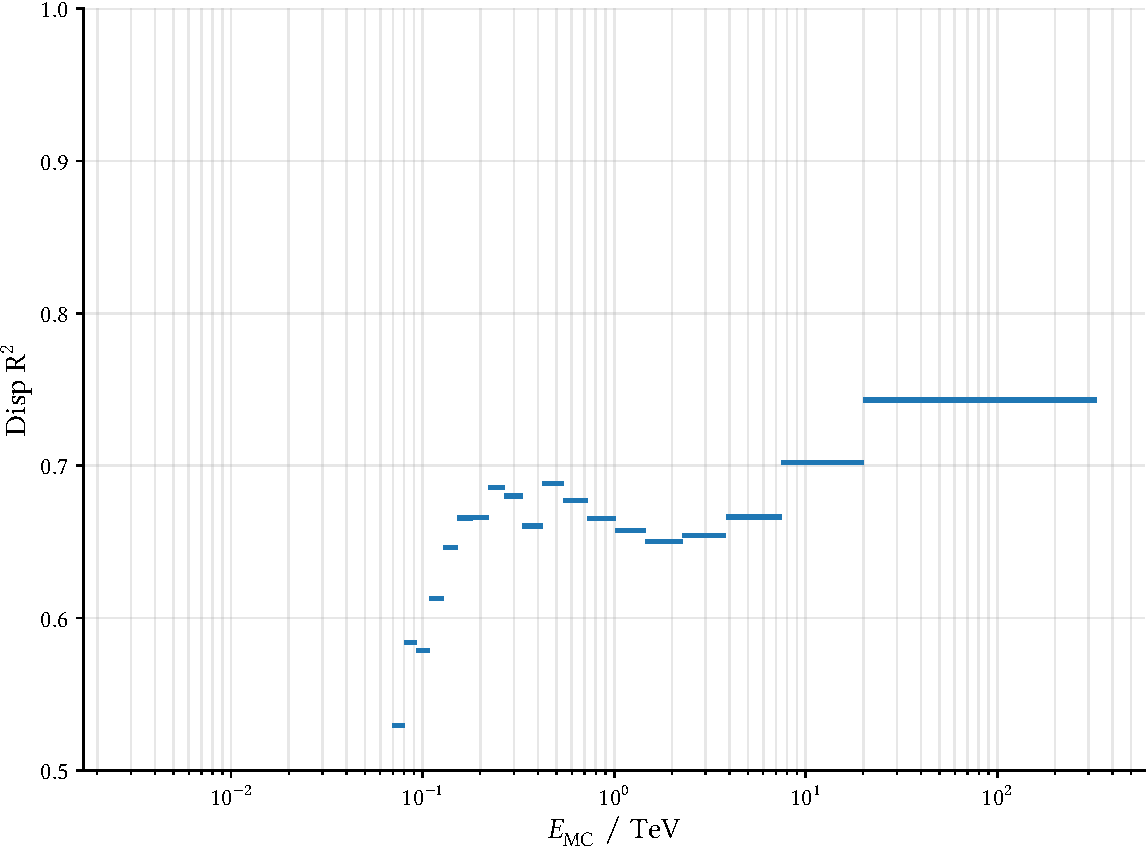
\includegraphics[width=0.9\linewidth]{../analysis/plots/disp_test_mono_lst_r2_equal_filled.pdf} 
        \caption{R2-Score for the DISP-estimation}
    \end{subfigure}
    \begin{subfigure}{0.45\textwidth}
        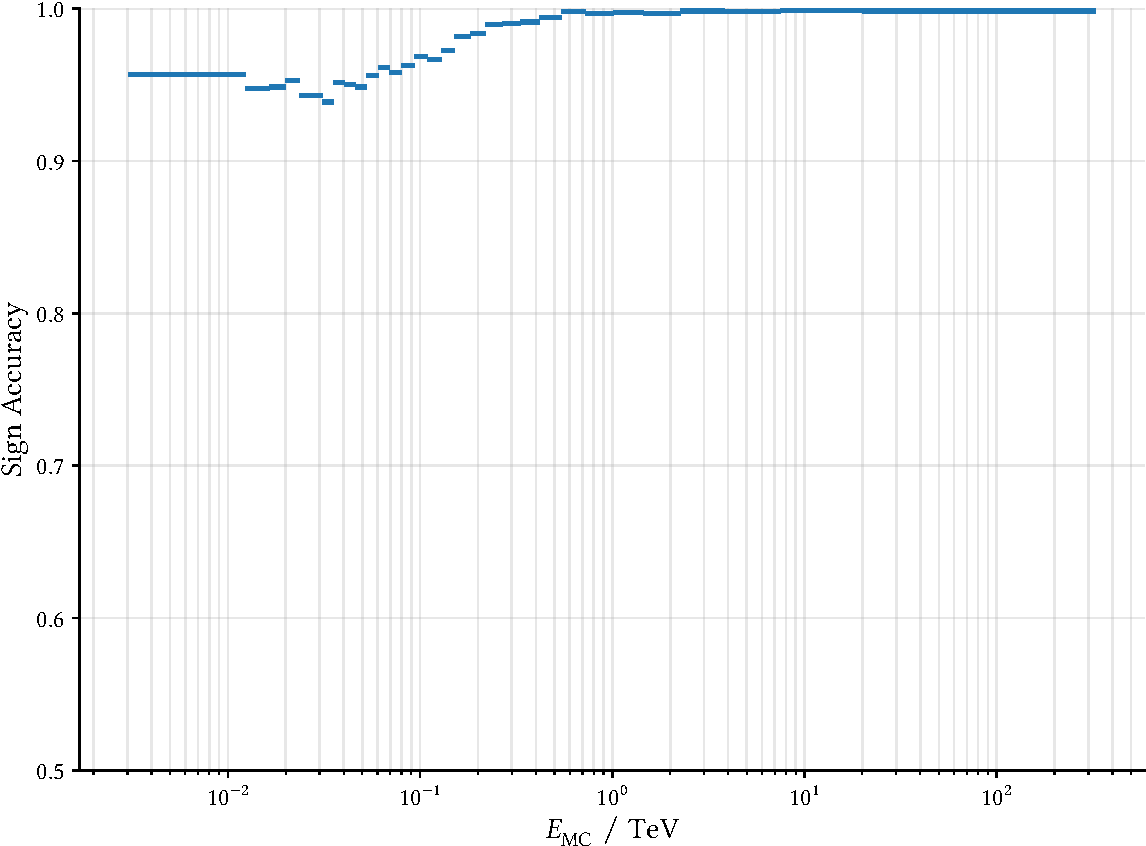
\includegraphics[width=0.9\linewidth]{../analysis/plots/disp_test_mono_lst_acc_equal_filled.pdf}
        \caption{SIGN-accuracy}
    \end{subfigure}
    \caption{Performance of the DISP- and SIGN-estimation algorithm on the test-dataset.}
    \label{fig:disp_test_perf}
\end{figure}

\begin{figure}
    \begin{subfigure}{0.45\textwidth}
        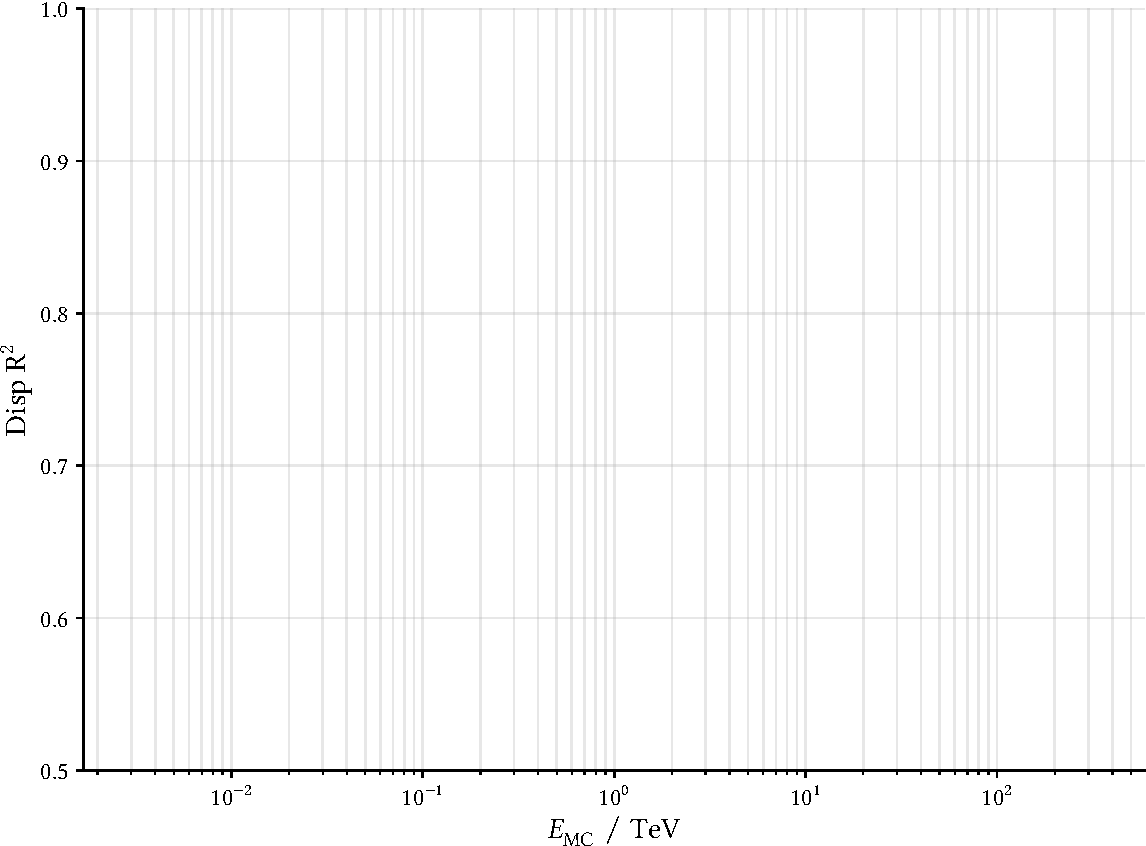
\includegraphics[width=0.9\linewidth]{../analysis/plots/disp_gamma_mono_lst_r2_equal_filled.pdf} 
        \caption{R2-Score for the DISP-estimation}
    \end{subfigure}
    \begin{subfigure}{0.45\textwidth}
        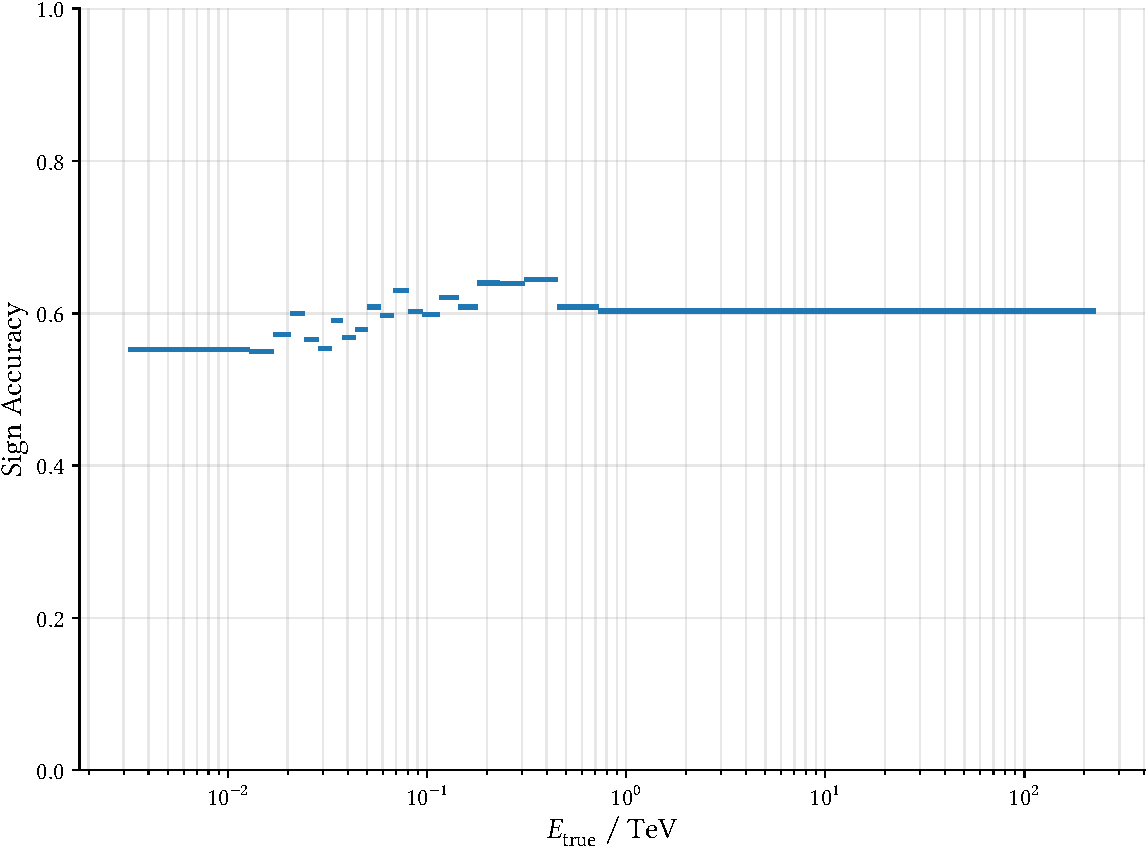
\includegraphics[width=0.9\linewidth]{../analysis/plots/disp_gamma_mono_lst_acc_equal_filled.pdf}
        \caption{SIGN-accuracy}
    \end{subfigure}
    \caption{Performance of the DISP- and SIGN-estimation algorithm on the pointlike dataset..}
    \label{fig:disp_gamma_perf}
\end{figure}

Looks decent, energy obviously limited bc LST.
